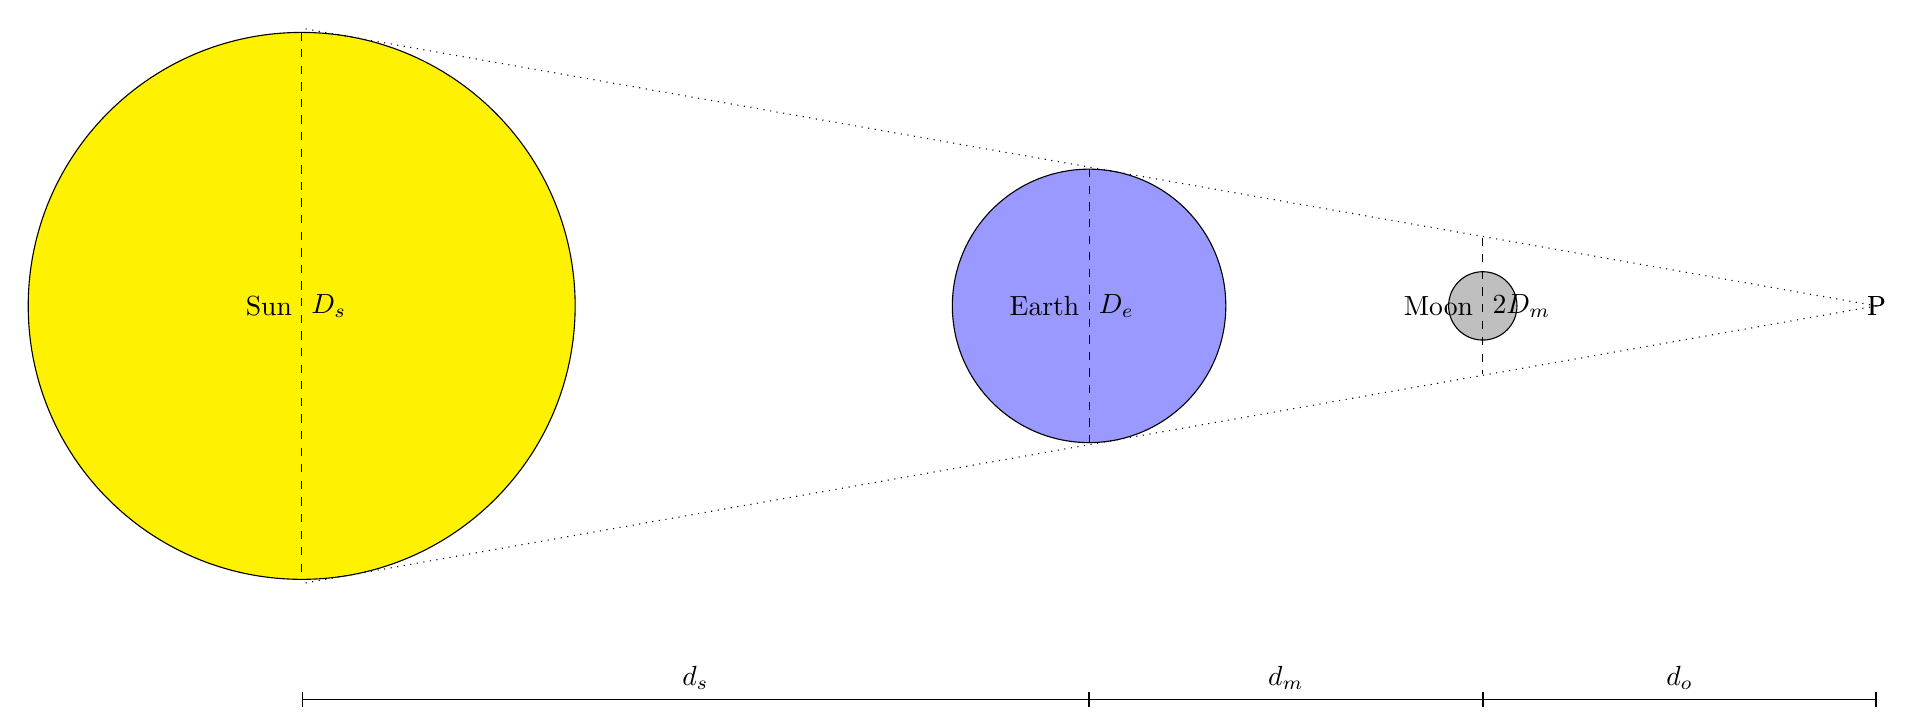
\begin{tikzpicture}[scale=1.0]

\def\eclipseangle{20}

% Sun 
\pgfmathparse{20*sin(10)}
\let\sunradius\pgfmathresult
\filldraw[fill=yellow] (0,0) circle (\sunradius) node[left] {Sun};
\draw[black,dashed] (0,\sunradius) -- (0,-\sunradius) node[midway,right] {$D_s$};

% Earth
\pgfmathparse{10*sin(10)}
\let\earthradius\pgfmathresult
\filldraw[fill=blue!40] (10,0) circle (\earthradius) node[left] {Earth};
\draw[black,dashed] (10,\earthradius) -- (10,-\earthradius) node[midway,right] {$D_e$};

% Moon
\pgfmathparse{5*sin(10)}
\let\moonradius\pgfmathresult
\filldraw[fill=gray!50] (15,0) circle (\moonradius/2) node[left] {Moon};
\draw[black,dashed] (15,\moonradius) -- (15,-\moonradius) node[midway,right] {$2D_m$};

% angle
\pgfmathparse{20*tan(10)}
\let\anglesize\pgfmathresult
\draw[dotted] (20,0) node {P} -- (0, \anglesize);
\draw[dotted] (20,0) node {P} -- (0, -\anglesize);

% distances
\draw[|-|] (0,-5) -- (10,-5) node[midway, above] {$d_s$};
\draw[|-|] (10,-5)--(15,-5) node[midway, above] {$d_m$};
\draw[|-|] (15,-5)--(20,-5) node[midway, above] {$d_o$};

\end{tikzpicture}